\chapter{Background}
\label{chap:background}
\textit{\hspace{0.5cm}This chapter introduces the background knowledge of this thesis, including information about Web Application Firewall, Machine Learning Models, HTTP request, Natural Language Processing, and Deep Neural Networks.}
\minitoc

\section{Web Application Firewall} 
\label{sec:waf}
\hspace{0.5cm}A Web Application Firewall helps protect web applications by filtering and monitoring HTTP traffic between a web application and the Internet. It typically protects web applications from attacks such as cross-site forgery, cross-site-scripting (XSS)\index{XSS}, file inclusion, and SQL injection\index{SQLi}, among others. 
\subsection{Definition}
\label{subsec:waf_def}
\hspace{0.5cm}WAF\index{WAF} stands for \textbf{Web Application Firewall}. This firewall solution commonly monitors data packets and filters them for the presence of malware or viruses. It performs the data monitoring/filtering for to and from data packets.  

The WAF tool can be distributed using network-based, cloud-based, or host-based architectures. It needs a reverse proxy to make sure that one or more web apps are in front of it while facing forward. It can be utilized either alone or in conjunction with other applications. WAF may function at a lower level or a higher level depending on the requirement\footnote{\label{wallarm} Wallarm. \textit{WAF Meaning}. \url{https://www.wallarm.com/what/waf-meaning}}.


\subsection{The functionality of WAF}
\label{subsec:waf_work}
\hspace{0.5cm}As previously stated, WAF is deployed at the application layer and serves as a two-way firewall. At work, WAF monitors HTTP or HTTPS traffic entering or exiting a specific web app. When WAF detects a malicious object in the traffic, it activates and destroys it. Figure 2.1 demonstrates how WAF works, legitimate users (top-left and bottom-left) are permitted access to the server with a WAF enabled, but attackers (middle-left) are prevented from doing so.
\begin{figure}[ht]
   
	\centering
	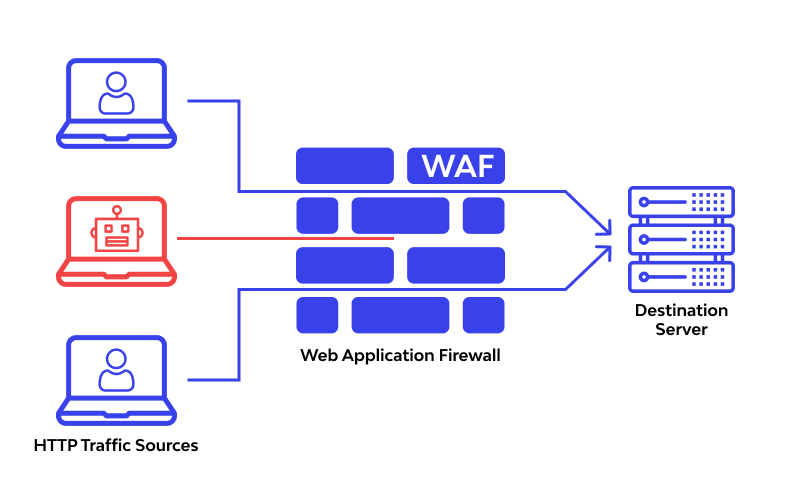
\includegraphics[width=\linewidth, height=6.5cm,keepaspectratio]{figures/wallarmwaf.png}
	\caption{How does WAF work (source: \url{https://www.wallarm.com/what/waf-meaning})}\label{Fig:Data1}
  
\end{figure} 

\newpage
WAF predefined what is malicious and what is not to make the process easier. WAF adheres to these guidelines throughout the process. WAF primarily analyzes the GET and POST portions of HTTP traffic. GET retrieves data from the server, whereas POST directs data to the server to change its original state\footnote{Wallarm. \textit{WAF Meaning}. \url{https://www.wallarm.com/what/waf-meaning}}.

% \footnoteref{wallarm}.


\subsection{Differences between WAF and firewall}
\label{subsec:versus}
\hspace{0.5cm}In the modern era of sophisticated cyberattacks and digital innovation, it is essential for organizations to understand the threats they face and what their security measures protect them from. Understanding the value of and distinctions between WAF\index{WAF} security and network firewall security is vital for preventing online attacks and other types of network intrusions\footnote{Fortinet. \textit{WAF vs. Firewall: Web Application and Network Firewalls}. 
\url{https://www.fortinet.com/resources/cyberglossary/waf-vs-firewall}}.

A web application firewall (WAF) protects web applications by intercepting Hypertext Transfer Protocol (HTTP) traffic. This is distinct from a traditional firewall, which acts as a wall between external and internal network traffic.

A WAF stands between external users and web applications to track all HTTP traffic. It then identifies and stops harmful requests from entering users or apps on the web. As a result, WAFs protect key company online applications and servers from zero-day threats and other application-layer attacks. This becomes highly critical as firms invest in new digital efforts, which could expose new web apps and APIs to attacks.

A network firewall guards a secure local-area network against unwanted access to reduce the risk of assaults. Its goal is to distinguish a safe zone from a less secure zone and to control communication between the two. Without it, every device that has a public IP address is exposed to the outside network and potentially vulnerable to attack.

The layer of security that WAF and network-level firewalls operate on is the primary technological distinction between them. Attacks at OSI model Layer 7, or the application level, are protected by WAFs. This covers URL assaults, cookie manipulation, SQL injection\index{SQLi}, and attacks against JavaScript, ActiveX, and Ajax applications. They also target HTTP and HTTPS, the web application protocols that link web browsers and web servers. Network firewalls secure data transfer and network traffic at OSI model Layers 3 and 4. This covers assaults on the Domain Name System (DNS) and File Transfer Protocol (FTP), as well as Telnet, Secure Shell (SSH), and Simple Mail Transfer Protocol (SMTP). The following figure (Figure 2.2) displays the attacks which can be blocked by network firewall and WAF.
\begin{figure}[ht]
	\centering
	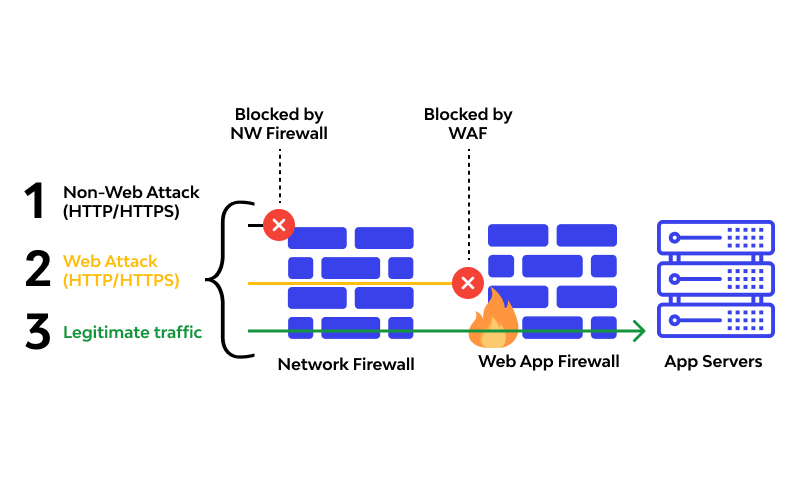
\includegraphics[width=\linewidth, height=7cm,keepaspectratio]{figures/waf3.png}
	\caption{WAF and network firewall block attacks (source: \url{https://www.wallarm.com/what/waf-meaning})}
\end{figure}
\newpage
It's critical to pick a suitable network firewall or WAF\index{WAF} to protect against all of the risks that may be present. Businesses cannot be protected from web page attacks by a network firewall alone; WAF capabilities are the sole means of defense. Business organizations risk leaving their larger network vulnerable to attack due to web application vulnerabilities without an application firewall. A WAF cannot protect from attacks at the network layer, so it should supplement a network firewall rather than replace it. Network-based and web-based solutions operate at several layers and protect from multiple types of traffic. As a result, they perform best together rather than against one another. A network firewall usually protects a wider range of traffic types, but a WAF deals with a specific threat that a conventional strategy cannot handle. Having both options is therefore advisable, especially if a company's operating systems and the web interact frequently.
\subsection{False positive}
\subsubsection{Definition}
\hspace{0.5cm}An alert produced when there is no real danger is known as a false positive\index{False positive} (FP). In other words, it serves as a warning indicator but ultimately proves to be a false alarm. False positives may appear to be innocuous annoyances, but they can have harmful effects\footnote{Hannah Brice. \textit{The Dangers of False Positives in Cybersecurity and how to avoid them}. Oct 2022. 
\url{https://www.lupovis.io/the-dangers-of-false-positives-in-cybersecurity-and-how-to-avoid-them/}}.
For instance, when it discovers unusual behavior on a network, an intrusion detection system (IDS) may send out an alert. However, additional research reveals that the behavior is harmless—a false positive. For IT security teams who have to waste time looking into them, they are frequently the result of wrong settings or overly vigilant security software.
\newpage
Handling a large number of notifications is something that all WAF\index{WAF} specialists have experience with. They're probably also wasting a ton of time sorting out false positives from these warnings. Attacks are to be stopped, while valid traffic is to be allowed to pass through the WAF. False positive incidents clog the alerts feed and, worse yet, block legitimate traffic. A few false positive incidents happen because of flaws or poor application design. A WAF rule that is too general or doesn't fit the site's operation may trigger additional events\footnote{A. Lerner, N. Avital, S. Margel. 
\textit{Alert fatigue - introducing false positives in WAF}. Aug 2020.
\raggedright\url{https://www.imperva.com/blog/avoid-alert-fatigue-how-to-automatically-get-rid-of-waf-false-positive/}}.
\subsubsection{The risks of false positive} 
\hspace{0.5cm}Any expanding company will worry about scalability, and expanding development processes presents several difficulties. Small-scale development still frequently uses ad hoc toolkits and manual procedures, while the former can still produce too many false positives\index{False positive}.

The number of false positives can expand exponentially, and it is hard to handle them all manually, as upgrades, products, and workloads all continue to multiply.

There may be substantial financial repercussions as well. It can take too long to investigate reports that turn out to be false positives, which can result in delays and a possible loss of money and business possibilities.

Due to the overwhelming amount of false positives, staff members could grow accustomed to ignoring reports, increasing the likelihood that an actual vulnerability will go unnoticed and enter the production application, again with very costly results\footnote{Ritika Singh. \textit{The Risks Of False Positives With Web Application Firewalls}. Sep 2021. \raggedright\url{https://www.indusface.com/blog/the-risks-of-false-positives-with-web-application-firewalls/}}.


\section{HTTP request}
\subsection{Normal request}
\hspace{0.5cm}HTTP request is information sent from the client to the server, to ask the server to find or process some information and data that the client wants. The HTTP request can be a text file in the form of XML or JSON that both can understand. Here is an HTTP request using the POST method (Figure 2.3).
\begin{figure}[ht]
	\centering
	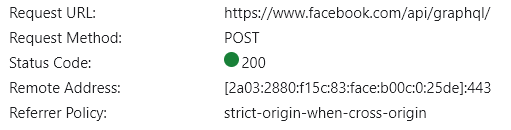
\includegraphics[width=\linewidth, height=3cm,keepaspectratio]{figures/normal request.png}
	\caption{Normal HTTP request using POST method}
\end{figure}

\hspace{0.5cm}An HTTP request consists of.
\begin{itemize}
	\item \textbf{Request line.} It begins with a method token, followed by the Request-URI and the protocol version, and ending with CRLF.
	\item \textbf{Body request.} It can be plain text, HTML, XML, JSON, Javascript, or a set of form-data key-value pairs.
\end{itemize}
\subsubsection{Request line}
\hspace{0.5cm}Request line is the first line of an HTTP request. It includes.
\begin{itemize}
	\item \textbf{HTTP method.} There are many types, but the most common are GET and POST.
	\item \textbf{URI (Uniform Resource Identifier).} It helps identify the resources requested by the client.
	\item \textbf{HTTP version.} The version of the HTTP protocol.
\end{itemize}
\subsubsection{Body request}
\hspace{0.5cm}Allows the client to send additional requests that the server needs to do, such as creating or updating data that cannot be passed on the Header Parameters. Request body is often used in POST, PUT, PATCH methods.
\subsection{Malicious request}
\hspace{0.5cm}Malicious traffic or malicious network traffic is any suspicious link, file or connection that is being created or received over the network. Malicious traffic is a threat with an organization's security or may compromise personal computers.

An example of a request used to attack Facebook is a cross-site scripting (XSS) attack (Figure 2.4). In this attack, a hacker can use a malicious HTTP request to inject JavaScript code into Facebook websites. When a user visits Facebook's website, JavaScript code is executed and allows the hacker to obtain the user's logins, transactions, and personal information.

\begin{figure}[ht]
	\centering
	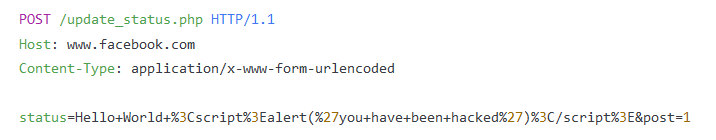
\includegraphics[width=\linewidth, height=7cm,keepaspectratio]{figures/malicious request.png}
	\caption{Malicious HTTP request used to attack Facebook}
\end{figure}

In it, the status field contains malicious HTML and JavaScript characters. When a user visits Facebook's website, this JavaScript code is executed and displays a malicious warning on the user's screen.

This can cause unsuspecting users to log into their accounts. Upon successful login, the user's credentials will be captured and used by the hacker to access their account and perform other malicious activities.


\section{Natural processing language}
\hspace{0.5cm}The field of computer science known as \emph{Natural Language Processing} (NLP)\index{NLP} is more particularly the branch of artificial intelligence (AI) that is concerned with providing computers the ability to understand spoken and written language like that of humans. Its practical applications include spam detection, translation, and sentiment analysis.

NLP blends statistical, machine learning, and deep learning models with computational linguistics—rule-based modeling of human language. With the use of these technologies, computers are now able to process human language in the form of text or audio data and fully ``understand'' what is being said or written, including the speaker's or writer's intentions and sentiments.

\subsection{Tokenization}
\hspace{0.5cm}Tokenization\index{Tokenization} is used in natural language processing to split paragraphs and sentences into smaller units that can be more easily assigned meaning. The first step of the NLP process is gathering the data (a sentence) and breaking it into understandable parts (words). 

There are 3 types of tokenization\index{Tokenization}.
\begin{itemize}
	\item \textbf{Word tokenization.} The most used type of tokenization is word tokenization. It employs delimiters (characters like `,' or `;' or ``,'') to divide the data into its corresponding words when there are natural breaks, like pauses in voice or spaces in the text. Although this is the simplest method for breaking up voice or text into component pieces, it has several disadvantages.  
	\item \textbf{Character tokenization.} Tokenization of characters was developed to solve some of the problems associated with word tokenization. It entirely splits text into characters rather than dividing it up into words. In contrast to word tokenization, this enables the tokenization process to maintain information about OOV terms.
	\item \textbf{Sub-word tokenization.} Similar to word tokenization, sub-word tokenization uses specific linguistic rules to further dissect individual words. They often use cutting-off affixes as one of their main tools. Prefixes, suffixes, and infixes can aid programs in comprehending the function of a word because they alter the basic meaning of words. This can be particularly helpful for terms not in your lexicon because figuring out an affix can provide a program with more understanding of how unfamiliar words work.  
\end{itemize}

\subsection{Vectorization}
\hspace{0.5cm}Vectorization\index{Vectorization} is a classic approach to converting input data from its raw format (i.e. text) into vectors of real numbers which is the format that ML models support. 
In machine learning, vectorization is a step in feature extraction. The idea is to get some distinct features out of the text for the model to train on, by converting text to numerical vectors.

Some vectorization techniques used in this thesis.
\begin{itemize}
	\item \textbf{TF-IDF.} It is a numerical statistic that's intended to reflect how important a word is to a document.
	\item \textbf{Word2Vec.} In a nutshell, this approach uses the power of a simple Neural Network to generate word embeddings. 
\end{itemize}


\section{Machine learning models} 

\label{sec:machine_model}
\hspace{0.5cm}In this thesis, we are using two machine learning algorithms to train the model: \textit{Logistic Regression} and \textit{Convolutional Neural Network}.
\subsection{Logistic regression}
\label{subsec:logistic_regression}
\hspace{0.5cm}One of the most used machine learning algorithms for binary classification is logistic regression\index{Logistic regression}. A logit function is used to forecast the likelihood that a binary outcome will occur. Given that it uses the log function to estimate outcome probabilities, it is a specific example of linear regression.

We turn the result into a categorical value using the activation function (sigmoid). Logistic regression has a wide range of applications, including the detection of fraud, spam, and other conditions.

Within machine learning, logistic regression belongs to the family of supervised machine learning models. It is also considered a discriminative model, which means that it attempts to distinguish between classes (or categories)\footnote{Dinesh Kumawat. \textit{Introduction to Logistic Regression - Sigmoid Function, Code Explanation}. Jan 2021. \raggedright\url{https://www.analyticssteps.com/blogs/introduction-logistic-regression-sigmoid-function-code-explanation}}.
\subsubsection{Logistic regression model}
\hspace{0.5cm}Predictive output of Linear Regression is displayed in (2.1).
\begin{align}
	f(x) = w^T x
\end{align}
\hspace{0.5cm}The predictive output of logistic regression is generally written as (2.2).
\begin{align}
	f(x) = \theta(w^T x)
\end{align}
where $\theta$ is called the logistic function. The logistic function in linear regression is a type of sigmoid, a class of functions with the same specific properties.
\subsubsection{Sigmoid Function}
\hspace{0.5cm}Sigmoid is a mathematical function that takes any real number and maps it to a probability between 1 and 0.
The formula of the sigmoid function is shown in (2.3).
\begin{align}
    f(x) = \frac{1}{1 + e^{-x}} \triangleq \sigma(x)
\end{align}

As a result of the sigmoid function's S-shaped graph (displayed in Figure 2.5), the probability increases as x approaches infinity and decreases as x approaches negative infinity. The model establishes a threshold that determines which binary variable corresponds to which probability range\footnote{
	Ayesha Naeem. \textit{What is sigmoid and its role in logistic regression?}. \url{https://www.educative.io/answers/what-is-sigmoid-and-its-role-in-logistic-regression}
}.

\begin{figure}[ht]
	\centering
	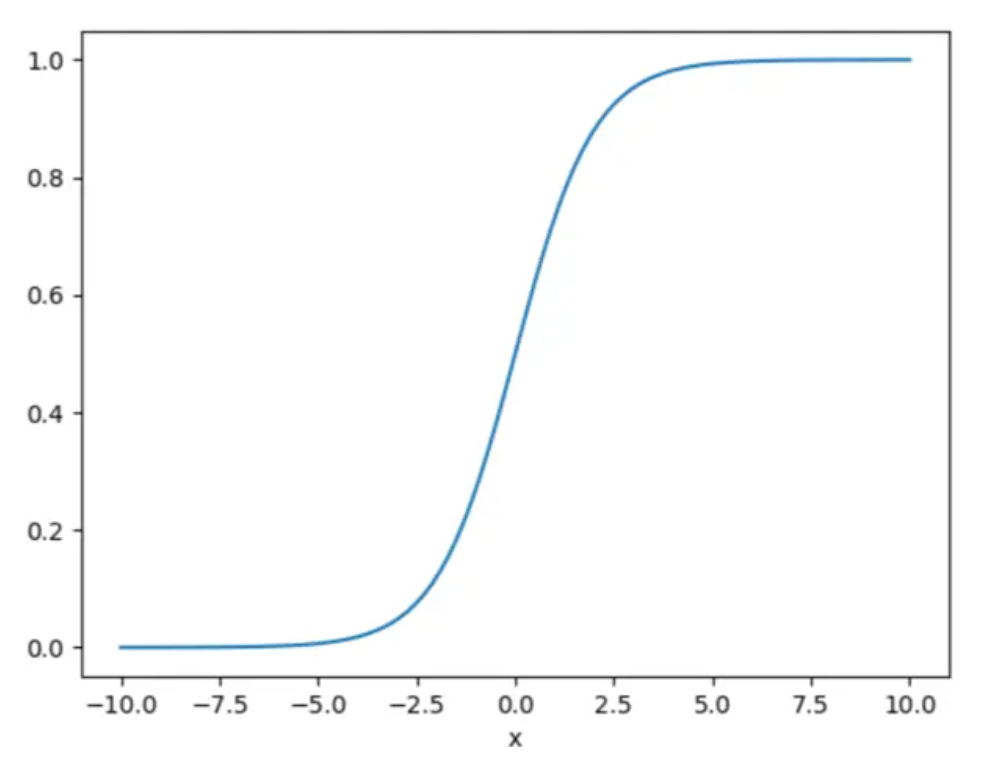
\includegraphics[width=\linewidth, height=6cm,keepaspectratio]{figures/sigmoid.PNG}
	\caption{Sigmoid function forms an S-shaped graph (source: \url{https://www.educative.io/answers/what-is-sigmoid-and-its-role-in-logistic-regression})}
\end{figure}

Suppose we have two possible outcomes, normal and abnormal, and have set the threshold as 0.5. A probability less than 0.5 would be mapped to the outcome abnormal, and a probability greater than or equal to 0.5 would be mapped to the outcome normal.

\subsubsection{Optimizing loss functions}
\hspace{0.5cm}The Stochastic Gradient Descent (SGD) algorithm will be used here. Loss function\index{Loss function} with only one data point (Equation 2.4).
\begin{align}
	J(w; x_i, y_i) = -(y_i \log {z}_i + (1-y_i) \log (1 - {z}_i))
\end{align}
\hspace{0.5cm}Using derivative, we have the expression shown in (2.5).
\begin{eqnarray}
	\frac{\partial J(w; x_i, y_i)}{\partial w} 
	&=& \frac{z_i - y_i}{z_i(1 - z_i)} \frac{\partial z_i}{\partial w} 
\end{eqnarray}
\hspace{0.5cm}To make this expression more compact and beautiful, we will find the function 
$z = f(w^T x)$ such that the denominator cancels out. If set $s = w^T x$, we have (2.6).
\begin{align}
	\frac{\partial z_i}{\partial w} = \frac{\partial z_i}{\partial s} \frac{\partial s}{\partial w} = \frac{\partial z_i}{\partial s} x  
\end{align}
\hspace{0.5cm}Most intuitively, we will find the function $z = f(s)$ such that (2.7) happens.
\begin{align}
	\frac{\partial z}{\partial s} = z(1 - z)
\end{align}
to suppress the denominator in the expression (2.5). Expression in (2.7) will be equivalent to.
\begin{align}
    % & \frac{\partial z}{z(1-z)} = \partial s \\ 
	% \Leftrightarrow & (\frac{1}{z} + \frac{1}{1 - z})\partial z = \partial s \notag \\  
	% \Leftrightarrow & \log(z) - \log(1 - z) = s \notag \\ 
	% \Leftrightarrow & \log \frac{z}{1 - z} = s \notag \\
	% \Leftrightarrow & \frac{z}{1 - z} = e^s \notag \\
	% \Leftrightarrow & z = e^s (1 - z) \notag \\
	% \Leftrightarrow & 
	z = \frac{e^s}{1 +e^s} = \frac{1}{1 + e^{-s}} = \sigma(s) 
\end{align}

\subsubsection{Updated math formula for logistic sigmoid regression}
\hspace{0.5cm}From above equations, we have (2.9).
\begin{align}
    \frac{\partial J(w; x_i, y_i)}{\partial w} = (z_i - y_i)x_i 
\end{align}
\hspace{0.5cm}The updated formula (according to the SGD algorithm) for logistic regression\index{Logistic regression} is displayed in (2.10).
\begin{align}
    w = w + \eta(y_i - z_i)x_i
\end{align}


\section{Deep neural network}
\label{sec:deep_neural_network}
\hspace{0.5cm}With their excellent results, broad applicability, and vast growth potential, neural networks are currently the most advanced advancement in artificial intelligence. \textit{Feedforward Neural Networks }(FNN) and \textit{Convolutional Neural Networks} (CNN)\index{CNN} are widely used to make predictions with independent data input. In CNN (Figure 2.6), each input image is passed through convolutional layers (Filters, Pooling, and Fully-connected layers) to extract features before being classified using the Softmax\index{Softmax} function\footnote{Softmax function:$ \sigma (\overrightarrow{z})_i \: = \: (e^{z_i})/ \sum_{j=1}^{K} e^z_i  $}.
\begin{figure}[ht] 
	\centering
	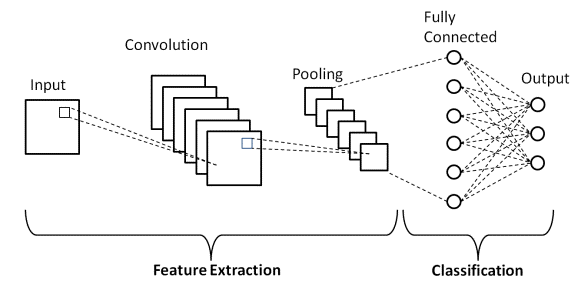
\includegraphics[width=\linewidth, height=6cm,keepaspectratio]{figures/CNN.png}
	\caption{CNN architecture (source: \url{https://www.upgrad.com/blog/basic-cnn-architecture/})}
\end{figure}	

\newpage
\emph{Layers}\index{Layer (Neural Network)} are the building components of deep neural networks\index{Deep Neural Network} such as CNN\index{CNN} and others. A layer is a broad phrase that refers to a group of ``nodes'' that function together at a given level within a neural network. Layers are classified into three types: \emph{input layer},\emph{ hidden layers}, and \emph{output layers}.

The \emph{input layer} contains raw data (each variable as a ``node'').
In neural networks, black magic happens in the \emph{hidden layer}(s). By minimizing an error/cost function, each layer attempts to learn different elements of the data. The context of ``image recognition'', such as a face, is the most intuitive way to understand these levels. The first layer may learn edge detection, the second eye, the third nose, and so on. This isn't exactly what's going on, but the idea is to split the problem down into components that different levels of abstraction can piece together, much to how our own brains work (hence the name neural networks).

The \emph{output layer} is the simplest, usually consisting of a single output for classification problems. Even though it is a single ``node'', it is nevertheless regarded as a layer in a neural network because it might contain numerous nodes. We use six types of layers given by the TensorFlow\index{TensorFlow} framework in this thesis: \textbf{Embedding} layer\index{Embedding layer}, \textbf{Conv1D} layer\index{Conv1D layer}, \textbf{MaxPooling1D} layer\index{MaxPooling1D layer}, \textbf{Dropout}\index{Dropout layer} layer, \textbf{Flatten} layer \index{Flatten layer}, and \textbf{Dense} layer\index{Dense layer}.

\subsection{Embedding layer}
\hspace{0.5cm}A class of methods for encoding words and documents using a dense vector representation is known as word embedding. It is an advance over the conventional bag-of-words\index{Bag-of-words} encoding techniques, in which each word was represented by a big sparse vector, or a complete vocabulary was represented by scoring each word within the vector. Due to the enormous vocabulary and the fact that most words and documents were represented by large vectors largely made up of zero values, these representations were sparse. In contrast, words are represented in an embedding by dense vectors, where a vector is the word's projection into a continuous vector space.

On text data, neural networks can be applied using an \emph{embedding layer}\index{Embedding layer}. The input data must be integer encoded for each word to be represented by a different number. All of the words in the training dataset will have an embedding learned by the embedding layer, which is initialized with random weights. It is a flexible layer that can be used in a variety of ways, such as.
\begin{itemize}
	\item It can be used alone to learn a word embedding that can be saved and used in another model later.
	\item It can be used as part of a deep learning model where the embedding is learned along with the model itself.
	\item It can be used to load a pre-trained word embedding model, a type of transfer learning.
\end{itemize}
\hspace{0.5cm}The embedding layer is defined as the first hidden layer of a network. It must specify 3 arguments.
\begin{itemize}
	\item $\textbf{input\_dim.}$ This is the size of the vocabulary in the text data. For example, if your data is integer encoded to values between 0 and 10, then the size of the vocabulary would be 11 words.
	\item $\textbf{output\_dim.}$ This is the size of the vector space in which words will be embedded. It defines the size of the output vectors from this layer for each word.
	\item $\textbf{input\_length.}$ This is the length of input sequences. For example, if all of the input documents are comprised of 1000 words, this would be 1000.
\end{itemize}
\hspace{0.5cm}Weights in the embedding layer are learned. If you save your model to file, this will include weights for the Embedding layer.

A 2D vector with one embedding for each word in the input word sequence (input document) is the result of the embedding layer.

\subsection{Conv1D layer}
\hspace{0.5cm}CNN\index{CNN} convolutional layers use learned filters to produce feature maps that represent the existence of certain features in the input.

A filter is created by concatenating several kernels, each of which is allocated to a different input channel. The difference between filters and kernels is always one dimension. For instance, filters in 1D convolutions are 2D matrices (basically, the kernels are a concatenation of 1D matrices). 
A kernel is a matrix that is slid across the input and multiplied by the input in order to enhance the output in a desired way.

Convolutional layers are particularly efficient, and stacking them in deep models enables the learning of high-order or more abstract characteristics, such as shapes or particular objects, by layers deeper in the model, while allowing layers near the input to learn low-level features, such as lines, at a faster rate. 

\emph{Conv1D layer}\index{Conv1D layer} produces a tensor of outputs by creating a convolution kernel and combining it with the layer input over a single spatial (or temporal) dimension.In TensorFlow\index{TensorFlow}, the input shape of this layer is a 3+ D tensor with shape: $batch\_shape + (steps, input\_dim)$, while the output shape is a 3+ D tensor with shape: $batch\_shape + (new\_steps, filters)$, $steps$ value might have changed due to padding or strides\footnote{
	Keras. \textit{Conv1D layer}. \url{https://keras.io/api/layers/convolution_layers/convolution1d/}
}.

\subsection{MaxPooling1D layer}
\hspace{0.5cm}The fact\index{MaxPooling1D layer} that convolutional layer feature maps preserve the exact location of input features is one of their limitations. This means that tiny movements in the position of the feature in the input image will result in a different feature map. This can happen with re-cropping, rotation, shifting, and other minor adjustments to the supplied image.

Downsampling is a popular strategy used in signal processing to solve this issue. In this case, a reduced resolution version of the input signal is produced, retaining the main structural features but excluding the small details that might not be as helpful.

By altering the convolution's stride over the image, convolutional layers can be used to do downsampling. Using a pooling layer is a more reliable and popular strategy.

In order to apply a pooling operation on feature maps, similar to a filter, pooling is conducted. The size of the pooling operation or filter, which is typically 2 $\times$ 2 pixels applied with a stride of 2 pixels, is smaller than the size of the feature map. This means that each feature map will always be compressed by a factor of 2, i.e., each dimension is cut in half, making each feature map only contain a quarter as many pixels or values.

Instead of being taught, the pooling operation is defined. A typical function used in the process of pooling is Max pooling, which works by calculating the maximum value for each patch of the feature map, and MaxPooling1D is applied for 1D temporal data. The max pooling is demonstrated in Figure 2.7.

\begin{figure}[ht]
	\centering
	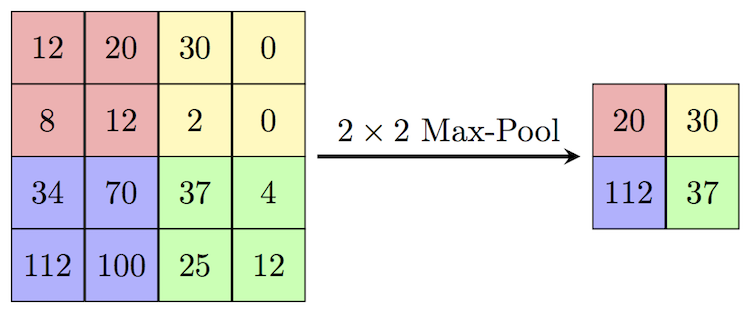
\includegraphics[width=\linewidth, height=4cm,keepaspectratio]{figures/maxpooling.png}
   \caption{Max pooling demonstration (source: \url{https://paperswithcode.com/method/max-pooling})}
\end{figure}

\subsection{Dropout layer}
\hspace{0.5cm}Dropout is a training method in which some neurons are ignored at random. They are ``dropped out'' in a random manner. It means that on the forward pass, their contribution to the activation of downstream neurons is momentarily removed, and on the backward pass, no weight updates are made to the neuron.

If neurons are randomly removed from the network during training, the remaining neurons will have to step in and handle the representation needed to produce predictions for the missing neurons. The network is believed to learn numerous independent internal representations as a result. Dropout procedure is demonstrated in Figure 2.8.
\begin{figure}[ht]
	\centering
	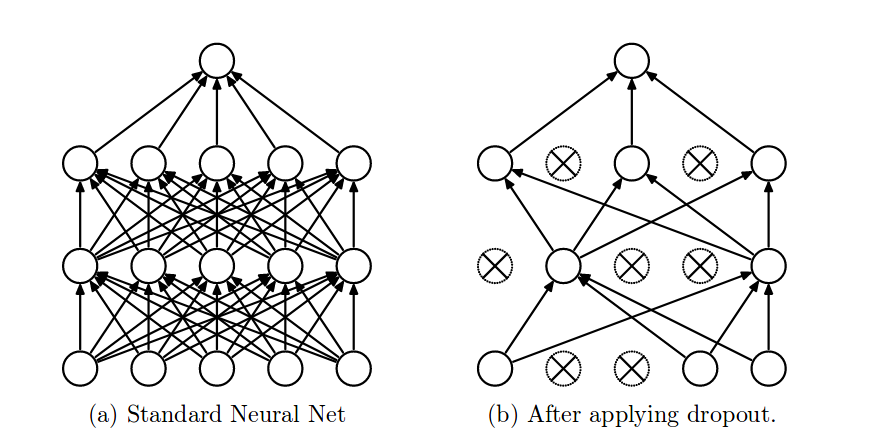
\includegraphics[width=\linewidth, height=6cm,keepaspectratio]{figures/dropout.png}
   \caption{Dropout demonstration (source: \url{https://laid.delanover.com/dropout-explained-and-implementation-in-tensorflow/})}
\end{figure}

\newpage
The result is a decrease in the network's sensitivity to the particular neuronal weights. As a result, the network is better able to generalize and is less prone to overfit the training set of data\footnote{
	Jason Brownlee. \textit{Dropout Regularization in Deep Learning Models with Keras}. Jul 2022. \url{https://machinelearningmastery.com/dropout-regularization-deep-learning-models-keras/}
}.
In Tensorflow\index{TensorFlow}, the \emph{dropout layer}\index{Dropout layer} randomly sets input units to 0 with a frequency of rate
at each step during training time. Inputs not set to 0 are scaled up by 1/(1 - rate)  (with rate is the fraction of the input units to drop) such that the sum over all inputs is unchanged\footnote{Keras. \textit{Dropout layer}. \url{https://keras.io/api/layers/regularization_layers/dropout/}}.
\subsection{Flatten layer}
\hspace{0.5cm}To\index{Flatten layer} enter data into the following layer, flattening converts the data to a 1-dimensional array. To construct a single, lengthy feature vector, the output of the convolutional layers is flattened. The last classification model, referred to as a fully-connected layer, is connected to it as well. In other words, the final layer is connected to the flattened, single-line representation of all the pixel data. The flatten procedure is displayed in Figure 2.9.
\begin{figure}[ht]
	\centering
	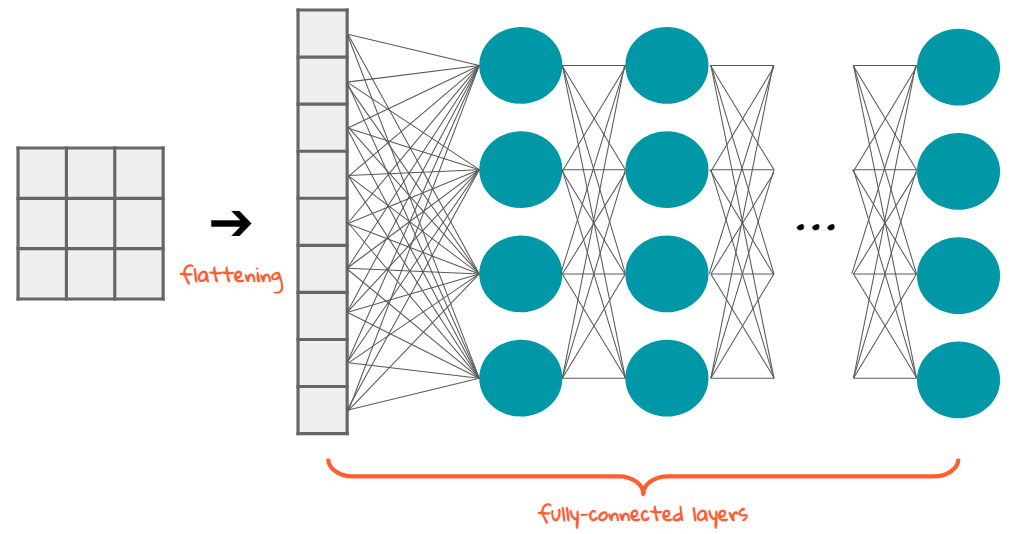
\includegraphics[width=\linewidth, height=5cm,keepaspectratio]{figures/flattening.png}
   \caption{Flattening demonstration (source: \url{https://towardsdatascience.com/the-most-intuitive-and-easiest-guide-for-convolutional-neural-network-3607be47480})}
\end{figure}
\newpage
\subsection{Dense layer}
\hspace{0.5cm}\emph{Dense layer}\index{Dense layer} is a neural network that has deep connection, meaning that each neuron in dense layer receives input from all neurons of its previous layer. The dense layer is found to be the most commonly used layer in the models.

The values utilized in the matrix are parameters that may be trained and updated with the aid of backpropagation, and the dense layer multiplies matrices and vectors. Dense Layer implements the following operation: \textit{output = activation(dot(input, kernel) + bias)}. The dense layer on the output performs \textit{dot product} of \textit{input tensor} (input) and \textit{weight kernel matrix} (kernel). A \textit{bias vector} (bias) is added and \textit{element-wise activation} (activation) is performed on output values. 

An `n' dimensional vector is produced as the dense layer's output. The vector can have its dimensions, rotation, scaling, and translation changed using a dense layer. 

\subsection{Gradient descent}
\label{subsec:gradient_descent}
\hspace{0.5cm}\emph{Gradient descent} is an optimization algorithm that is used to minimize a function by iteratively traveling in the direction of the steepest descent as defined by the gradient's negative. Gradient descent\index{Gradient descent} is used in machine learning\index{Machine learning (ML)} to update the parameters of our model, especially weights in neural networks. Gradient descent is demonstrated in Figure 2.10. \\ 
\begin{figure}[ht]
	\centering
	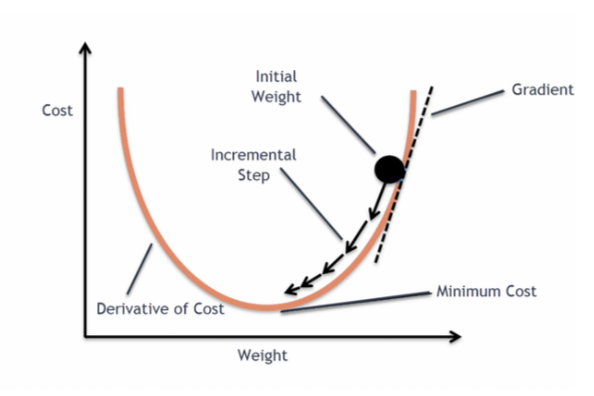
\includegraphics[width=\linewidth, height=6cm,keepaspectratio]{figures/gradient descent.png}
   \caption{Gradient descent demonstration (source: \url{https://www.analyticsvidhya.com/blog/2020/10/how-does-the-gradient-descent-algorithm-work-in-machine-learning/})}
\end{figure}

The objective of gradient descent is to minimize the cost function, or the error between predicted and actually, much like the purpose of determining the line of best fit in linear regression. It needs two data points to perform this: a direction and a learning rate. Future iterations' partial derivative calculations are determined by these variables, allowing the local or global minimum (i.e., point of convergence) to be reached gradually\footnote{IBM.\textit{What is gradient descent?}.\url{https://www.ibm.com/topics/gradient-descent}}.
\subsection{Learning Rate}
\label{subsec:learning_rate}
\hspace{0.5cm}The learning rate\index{Learning rate} is the size of each step in each gradient descent\index{Gradient descent} cycle. We can cover more territory per step with a high learning rate, but we risk overshooting the lowest spot because the slope of the hill is continually changing. We may reliably go in the direction of the negative gradient with a very low learning rate because we are recalculating it so frequently. A low learning rate is more exact, but calculating the gradient takes time, so we will take a long time to reach the bottom. An example of the learning rate is in Figure 2.11.
\begin{figure}[ht]
	\centering
	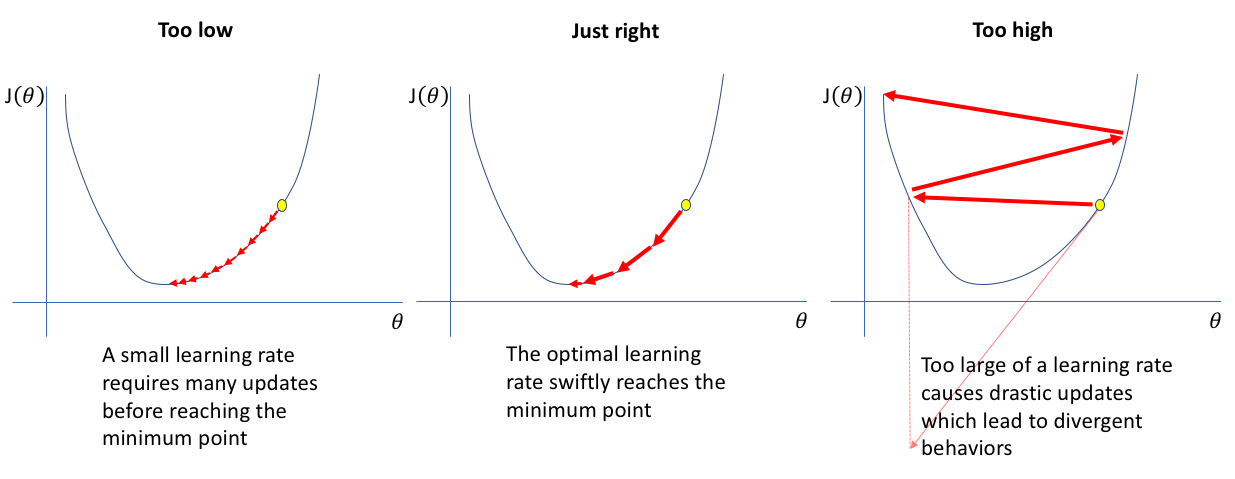
\includegraphics[width=\linewidth, height=6cm,keepaspectratio]{figures/learning rate.png}
   \caption{Learning rate (source: \url{https://www.jeremyjordan.me/nn-learning-rate/})}
\end{figure}

How quickly the model adapts to the challenge is determined by the learning rate. Given the smaller changes to the weights made with each update, lower learning rates necessitate more training epochs, whereas higher learning rates produce quick changes and necessitate fewer training epochs.

When the learning rate is too high, the model may converge too rapidly to an unsatisfactory answer, whereas when it is too low, the process may become stuck.

Choosing the learning rate appropriately is a difficult aspect in training deep learning neural networks. For the model, it can be the most crucial hyperparameter\footnote{Jason Brownlee. \textit{Understand the Impact of Learning Rate on Neural Network Performance}. Jan 2019. \url{https://machinelearningmastery.com/understand-the-dynamics-of-learning-rate-on-deep-learning-neural-networks/}}.

\newpage
\subsection{Loss function}
\label{subsec:loss_function}
\hspace{0.5cm}A loss function\index{Loss function} (or cost function) indicates how well the model predicts a given set of parameters. The loss function has its curve and gradients. The slope of this curve indicates how we should adjust our parameters to improve the model's accuracy\index{Accuracy}. If the cost ever rises, we must reduce the value of the learning rate\index{Learning rate}; if the cost falls slowly, we must increase the value of the learning rate. Figure 2.12 shows an example of loss function behavior based on the learning rate.
\begin{figure}[ht]
	\centering
	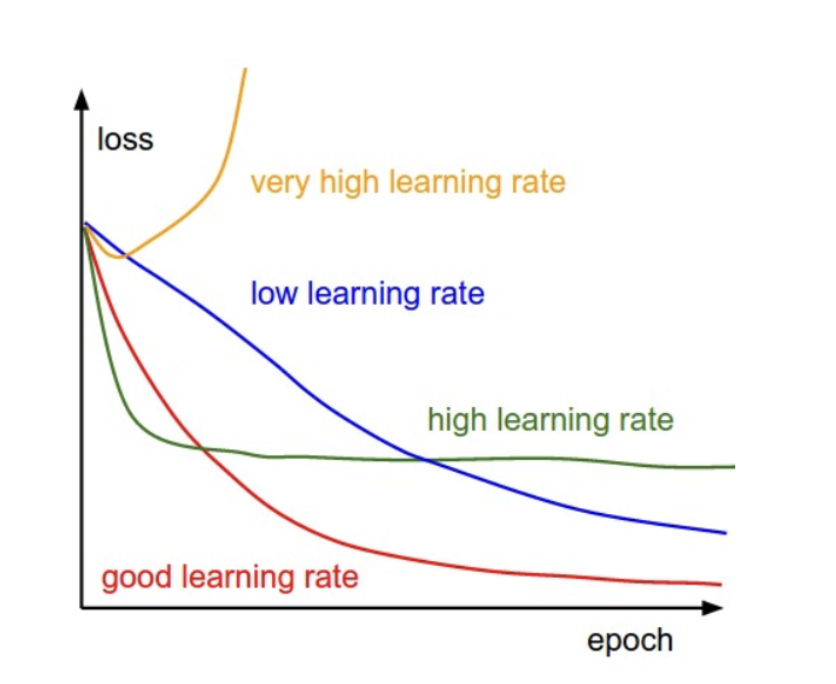
\includegraphics[width=\linewidth, height=7cm,keepaspectratio]{figures/loss function DL.png}
   \caption{Loss function behaviour with different learning rate (source: \url{https://www.researchgate.net/figure/Loss-function-is-changing-with-different-learning-rates-30_fig4_342657394})}
\end{figure}

\subsection{Gradient descent optimizer}
\label{gradient_optimizer}
\hspace{0.5cm}A\index{Gradient descent optimizer} method that computes adaptive learning rates\index{Learning rate} for each parameter is \textit{Adaptive Moment Estimation} (Adam). Adam\index{Adam (algorithm)}, like Adadelta and RMSprop, preserves an exponentially decaying average of past squared gradients $v_t$ in addition to an exponentially decaying average of past gradients $m_t$. Whereas momentum can be thought of as a ball rolling down a hill, Adam behaves more like a heavy ball with friction, preferring flat minima on the error surface. The decaying averages of past and past squared gradients, $m_t$ and $v_t$, are computed as follows (2.11).
\begin{align}
    m_t \: = \: \beta_1 m_{t-1} \: + \: (1-\beta_1)g_{t}\\
    v_t \: = \: \beta_2 v_{t-1} \: + \: (1-\beta_2)g^2_t \notag
\end{align}


$m_t$ and $v_t$ are estimates of the first moment (the mean) and the second moment (the uncentered variance) of the gradients respectively, hence the name of the method. As $m_t$ and $v_t$ are initialized as vectors of 0's, the authors of Adam\index{Adam (algorithm)} observe that they are biased towards zero, especially during the initial time steps, especially when the decay rates are small.
\begin{align}
    \hat{m}_t \: = \: \frac{m_t}{1\:-\:\beta^t_1} \\
 \hat{v}_t \: = \: \frac{v_t}{1\: - \: \beta^t_2} \notag
\end{align}



They then use these to update the parameters.
\begin{align}
\theta_{t+1} \: = \: \theta_t \: - \: \frac{\eta}{\sqrt{\hat{v}_t} \: +\: \epsilon} \hat{m}_t
\end{align}
